\documentclass[11pt,letterpaper]{article}
\usepackage{cogsys}
\usepackage{cogsysapa}
% \usepackage{apacite}
% \usepackage{graphicx}
\usepackage[T1]{fontenc}
\usepackage{times}
\usepackage[pdftex]{graphicx} % use this when importing PDF files

 % First page headings for accepted submissions.
\cogsysheading{X}{20XX}{1-6}{3/2015}{X/20XX}
 % First page headings for poster submissions.
%\cogsysposterheading{First}{2012}{1-18}

\ShortHeadings{Interactive Knowledge-Goal Reasoning}
              {B.\ Bengfort and M.\ Cox}

\begin{document}

\title{Interactive Knowledge-Goal Reasoning}

\author{Benjamin Bengfort}{bengfort@cs.umd.edu}
\address{Department of Computer Science, University of Maryland,
         College Park, MD 20742 USA}
\author{Michael Cox}{michael.cox@wright.edu}
\address{Wright State Research Institute,
         Beavercreek, OH 45431 USA}
\vskip 0.2in
 
\begin{abstract}
The goal of this paper is to provide a description for a question and answer system that uses mixed-initiative approaches to solve knowledge goals. This paper describes the problem in terms of two types of knowledge goals: simple and complex. It describes a collaborative, case-based reasoning framework for how a question/answer system would leverage both linked data and a casebase of prior examples to solve such problems.
\end{abstract}

\section{Introduction}

Much of the research related to automatically solving knowledge goals has focused on the human aspect: the parsing of a natural language question to a structured database query \cite{yahya_natural_2012,unger_template-based_2012,berant_semantic_2013}. These parsing approaches are able to rapidly solve simple knowledge goals, where the primary task is a retrieval from some structured knowledge base. Goals that ask "who", "what", "when" or "where" with a criteria set of concepts and expect an entity as a response benefit from these parsing approaches, as they are able to express layered criteria; for example the question "Who won the 1994 World Cup?" requires the ability to identify the \texttt{1994 FIFA World Cup}\footnote{https://www.freebase.com/m/012xwf} entity and to use semantic relationships to respond with an entity that is of type \texttt{Country}\footnote{https://www.freebase.com/location/country?schema=}. Even these simple knowledge goals can be complex, "Who was the King of England when Thomas Jefferson was President?" must be parsed to a chained query that involves implied entities like the United States of America.

Although impressive work is being done in the parsing task; these types of simple knowledge goal solutions are not able to solve complex knowledge goals including aggregations - "How many countries have won three consecutive gold medals in the same sport?", opinions - "What is the best restaurant in Boston?", or complex knowledge goals that require an explanation such as "why" or "how" questions. Because these simple knowledge goals focus on a single task, the retrieval of a unit piece of information from a database, they cannot be used to solve the variety of tasks that may be required to generally solve knowledge goals. Moreover, these questions do not take into account other important features such as context ("Is it raining outside?") and will always return the same answer for a repeated question regardless of how routine that question is ("Where should I go to dinner?").

However, complex knowledge goals can solved by decomposing the larger knowledge problem into sub goals that contribute some information to the solution. This decomposition represents a plan to solve the larger knowledge goal, and if the leaf nodes of knowledge acquisition plans are simple knowledge goals like structured data retrieval, then a system can be said to compute complex knowledge goals through the computationally tractable combination of simpler knowledge goals. Consider how a person might solve the knowledge goal "Can a crocodile complete a steeplechase?" They might first ask the question, "What is a Steeplechase?". Then upon discovering that a Steeplechase requires leaping over hurdles might ask the question, "How high can a crocodile jump?". Together the answers to these two simpler knowledge goals reveal that some Crocodiles might be able to leap the hurdles, but most cannot.

Goal driven natural language queries are therefore knowledge goals whose solution is a plan composed of simpler knowledge goals, the leaf nodes of which are computationally tractable tasks, either database queries or document retrieval. Computational systems that automatically solve goal driven natural language queries must formulate plans which take into account the context of the user (profile information, location, time, etc.) and must leverage a wide array of data sources to perform tasks. In this paper we will present the vision for such a computational system that makes use of case based reasoning in a mixed initiative environment to propose plans to the user then execute knowledge related tasks to arrive at the solution to complex knowledge goals. This type of system is adaptive and subject to goal changes, where the original knowledge goal is changed slightly as a result of following some solution plan creating goal trajectories.

\section{Knowledge Goals}

Knowledge goals represent the need to acquire information or data, to fill in gaps in the world knowledge of an entity or in the database of a system. Knowledge goals are important parts of any understanding system and in fact the planful execution of information retrieval is essentially a learning process that mimics how humans learn and adapt to new situations \cite{ram_goal-based_1991}. Intelligent information retrieval systems must make inferences, perform ambiguity resolution, add relevant context, and resolve gaps in knowledge. As such, knowledge goals are essential to natural language understanding systems that require similar tasks.

There are two broad classes of knowledge goals, related to the underlying solution task. \textit{Simple knowledge goals} can be represented as database queries, either as natural language questions that expect a factual response and should be parsed into a structured query language such as SQL or SPARQL. \textit{Complex knowledge goals} cannot be directly translated to a database query due to concept or task ambiguity, schema or type generalities, missing contextual information, or non-storage related expected results. Many complex knowledge goals should be solved instead by the development of an information retrieval plan whose sub goals are less complex than the original goal.

The complex knowledge goal that we will primarily consider in this paper is "What courses should I take next semester?". This task of this knowledge goal is to deliver a set of courses that the student will presumably register for. A question like this is routine, executed by same person on a regular interval, and common enough that a large casebase of plans to solve the question is readily available. To solve this knowledge goal, the system might respond with sub knowledge goals such as, "What days and times would you prefer?", "Are there any subjects you're interested in?", or "Do you have any academic requirements?". Responses to these questions will lead to simple knowledge goals that can be queried against a course catalog, e.g. "What economic courses are available on Monday and Wednesday?".

\subsection{Components of a Question}

Both simple and complex knowledge goals can be represented as natural language queries, however in order to begin the task of planning to solve a knowledge goal, either through the construction of a database query or a plan, the knowledge goal must be parsed into its components:

\begin{enumerate}
\item \textbf{Concept}: The concept related to the question including all of the involved entities, either directly specified or implied. The concept provides the question with a domain to search upon.
\item \textbf{Task}: The purpose of the question. Tasks are related to the categorization of the question, outlined in the taxonomy below, and are related to the motivation of the user. The task will determine the execution context of the knowledge goal solution.
\item \textbf{Context}: The user-specific context of the question provides a lot of information for refining the plan or resolving ambiguities. Context is often required in order to solve the question.
\end{enumerate}

Consider the question: "What was the score of the World Series?". This question is a simple knowledge goal because the task is a database retrieval for \texttt{result} property of the entity \texttt{2014 World Series}. The concept is the text "World Series" which must be resolved to an entity in the database, as well as the text "score" which indicates the object of query. The context implies that the most recent World Series score is required since none was specified in the text.

A complex knowledge goal, such as "Where should we go to dinner?" has a significant amount of associated context including the geographic location of the diner, the amount of time to make a decision before dinner, the number of diners, etc. The task is a plan to filter all restaurants in a particular location to a ranked list of suitable candidate choices, and therefore the concept is the general type \texttt{Restaurant} which must be inferred from the text "dinner". Plans to solve this particular complex knowledge goal would be associated with the properties of the concept such as rating, genre, price, etc.


\subsection{A Taxonomy of Questions}

Knowledge goals as described in \cite{ram_knowledge_1990} are presented with a categorization based on the task that they arise from. Here, we can see that the type of question may motivate the task required for planning and extend upon that taxonomy already given. Simple knowledge goals that can be automatically computed are as follows:

\textbf{Text Questions:} Questions related to both semantic or syntactic analysis of text, usually as a response to some ambiguity in the input or to resolve dependencies in the output. Tasks related to text questions include anaphora resolution or word sense disambiguation.

\textbf{Contextual Questions:} Questions designed to repair gaps in knowledge concerning the context of a question. Similar to text questions, these types of questions are "meta-questions" that are used to tailor the execution of a knowledge goal solution.

\textbf{Rhetorical Questions:} Questions that should not return an answer.

\textbf{Retrieval Questions:} A query that expects a single fact returned from the database. These types of questions may perform aggregations or filtering upon the knowledge base, but typically only return a single result or a small list of results.

Complex knowledge goals

\textbf{Explanation Questions:} Questions that require an explanation and return an explanatory data structure. Tasks include the detection and resolution of anomalies as well as the construction of an inferential or causal explanation.

\textbf{Relevance Questions:} These questions are designed to expand the current knowledge framework by adding relevance links between questions and related entities, answers or other questions. Relevance can be used in later processing as a shortcut to retrieval from a casebase.

\textbf{Socratic Questions:} Socratic questions return a question as an answer, or rather a plan that consists of knowledge goals that are designed to answer the larger question.

\textbf{Research Questions:} These types of questions are designed to add information to a knowledge base, either by adding facts or creating knowledge from other knowledge sources. The system should identify research questions based on unsatsifactory queries and add them to the system for later investigation.

\textbf{Routine Questions:} Questions that are routine are asked frequently or on a specific interval, however the required answer will differ based on the context or timing of the question and will most likely not return the same answer as a previous instance of the question.

The taxonomy of questions plays a large role in terms of the computational effectiveness of designing a system that can interactively plan and execute mixed-initiative, intelligent information retrieval. Many of these types of questions are task related

\subsection{Goal Trajectories}

\begin{figure}
	\centering
	    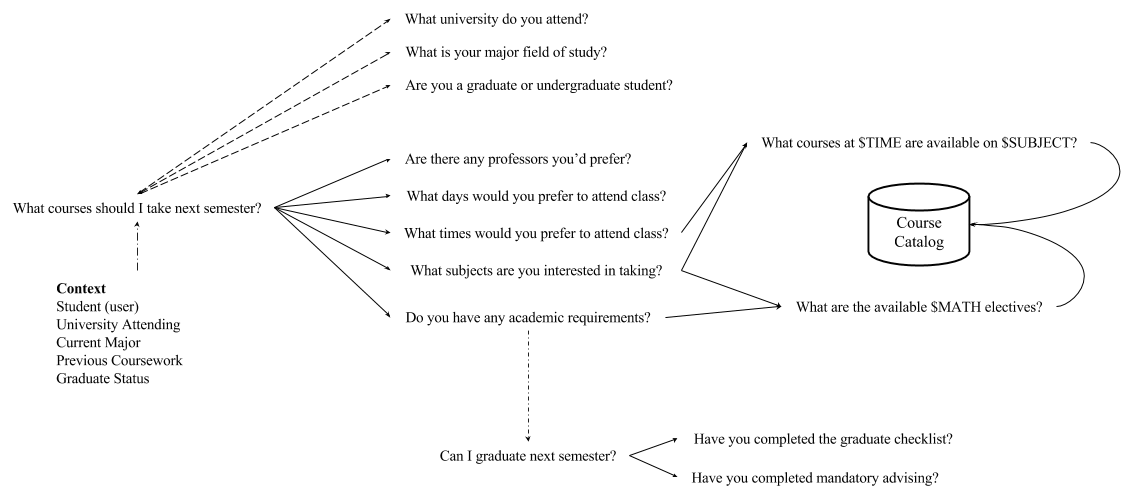
\includegraphics[width=\textwidth]{figures/simple_trajectory.png}
    \caption{\label{fig:simple_trajectory.png}A simple knowledge goal solution with trajectory change}
\end{figure}

Plans and knowledge goals are adaptable, subject to change as the system proceeds executing complex queries to discover knowledge and explanation \cite{munoz-avila_case-based_2008}. Goal trajectories can be influenced by other users in the system, either humans who are issuing similar queries and providing recommended goals through collaborative filtering \cite{hayes_case-based_2001} or via monitoring of automatic systems on new information or relevant data that has been added to the knowledge base. In either case, mixed-initiative goal changes can be seen as a planning problem that must be responsive to change \cite{cox_mixed-initiative_2007}.

% \newpage

\begin{acknowledgements}
\noindent
Please place your acknowledgements in an unnumbered section at the
end of the paper. Typically, this will include thanks to reviewers
who gave useful comments, to colleagues who contributed to the ideas,
and to funding agencies or corporate sponsors that provided financial
support.
\end{acknowledgements}

\vspace{-0.25in}

{\parindent -10pt\leftskip 10pt\noindent
\bibliographystyle{cogsysapa}
\bibliography{kgworkshop}

}

% Leave a blank line before the closing brace to ensure the final
% reference has the proper indentation.

\end{document}
